\documentclass[]{article}
\usepackage{lmodern}
\usepackage{amssymb,amsmath}
\usepackage{ifxetex,ifluatex}
\usepackage{fixltx2e} % provides \textsubscript
\ifnum 0\ifxetex 1\fi\ifluatex 1\fi=0 % if pdftex
  \usepackage[T1]{fontenc}
  \usepackage[utf8]{inputenc}
\else % if luatex or xelatex
  \ifxetex
    \usepackage{mathspec}
  \else
    \usepackage{fontspec}
  \fi
  \defaultfontfeatures{Ligatures=TeX,Scale=MatchLowercase}
\fi
% use upquote if available, for straight quotes in verbatim environments
\IfFileExists{upquote.sty}{\usepackage{upquote}}{}
% use microtype if available
\IfFileExists{microtype.sty}{%
\usepackage{microtype}
\UseMicrotypeSet[protrusion]{basicmath} % disable protrusion for tt fonts
}{}
\usepackage[margin=1in]{geometry}
\usepackage{hyperref}
\hypersetup{unicode=true,
            pdftitle={Case Study 3: Becoming a Databender},
            pdfborder={0 0 0},
            breaklinks=true}
\urlstyle{same}  % don't use monospace font for urls
\usepackage{color}
\usepackage{fancyvrb}
\newcommand{\VerbBar}{|}
\newcommand{\VERB}{\Verb[commandchars=\\\{\}]}
\DefineVerbatimEnvironment{Highlighting}{Verbatim}{commandchars=\\\{\}}
% Add ',fontsize=\small' for more characters per line
\usepackage{framed}
\definecolor{shadecolor}{RGB}{248,248,248}
\newenvironment{Shaded}{\begin{snugshade}}{\end{snugshade}}
\newcommand{\KeywordTok}[1]{\textcolor[rgb]{0.13,0.29,0.53}{\textbf{#1}}}
\newcommand{\DataTypeTok}[1]{\textcolor[rgb]{0.13,0.29,0.53}{#1}}
\newcommand{\DecValTok}[1]{\textcolor[rgb]{0.00,0.00,0.81}{#1}}
\newcommand{\BaseNTok}[1]{\textcolor[rgb]{0.00,0.00,0.81}{#1}}
\newcommand{\FloatTok}[1]{\textcolor[rgb]{0.00,0.00,0.81}{#1}}
\newcommand{\ConstantTok}[1]{\textcolor[rgb]{0.00,0.00,0.00}{#1}}
\newcommand{\CharTok}[1]{\textcolor[rgb]{0.31,0.60,0.02}{#1}}
\newcommand{\SpecialCharTok}[1]{\textcolor[rgb]{0.00,0.00,0.00}{#1}}
\newcommand{\StringTok}[1]{\textcolor[rgb]{0.31,0.60,0.02}{#1}}
\newcommand{\VerbatimStringTok}[1]{\textcolor[rgb]{0.31,0.60,0.02}{#1}}
\newcommand{\SpecialStringTok}[1]{\textcolor[rgb]{0.31,0.60,0.02}{#1}}
\newcommand{\ImportTok}[1]{#1}
\newcommand{\CommentTok}[1]{\textcolor[rgb]{0.56,0.35,0.01}{\textit{#1}}}
\newcommand{\DocumentationTok}[1]{\textcolor[rgb]{0.56,0.35,0.01}{\textbf{\textit{#1}}}}
\newcommand{\AnnotationTok}[1]{\textcolor[rgb]{0.56,0.35,0.01}{\textbf{\textit{#1}}}}
\newcommand{\CommentVarTok}[1]{\textcolor[rgb]{0.56,0.35,0.01}{\textbf{\textit{#1}}}}
\newcommand{\OtherTok}[1]{\textcolor[rgb]{0.56,0.35,0.01}{#1}}
\newcommand{\FunctionTok}[1]{\textcolor[rgb]{0.00,0.00,0.00}{#1}}
\newcommand{\VariableTok}[1]{\textcolor[rgb]{0.00,0.00,0.00}{#1}}
\newcommand{\ControlFlowTok}[1]{\textcolor[rgb]{0.13,0.29,0.53}{\textbf{#1}}}
\newcommand{\OperatorTok}[1]{\textcolor[rgb]{0.81,0.36,0.00}{\textbf{#1}}}
\newcommand{\BuiltInTok}[1]{#1}
\newcommand{\ExtensionTok}[1]{#1}
\newcommand{\PreprocessorTok}[1]{\textcolor[rgb]{0.56,0.35,0.01}{\textit{#1}}}
\newcommand{\AttributeTok}[1]{\textcolor[rgb]{0.77,0.63,0.00}{#1}}
\newcommand{\RegionMarkerTok}[1]{#1}
\newcommand{\InformationTok}[1]{\textcolor[rgb]{0.56,0.35,0.01}{\textbf{\textit{#1}}}}
\newcommand{\WarningTok}[1]{\textcolor[rgb]{0.56,0.35,0.01}{\textbf{\textit{#1}}}}
\newcommand{\AlertTok}[1]{\textcolor[rgb]{0.94,0.16,0.16}{#1}}
\newcommand{\ErrorTok}[1]{\textcolor[rgb]{0.64,0.00,0.00}{\textbf{#1}}}
\newcommand{\NormalTok}[1]{#1}
\usepackage{longtable,booktabs}
\usepackage{graphicx,grffile}
\makeatletter
\def\maxwidth{\ifdim\Gin@nat@width>\linewidth\linewidth\else\Gin@nat@width\fi}
\def\maxheight{\ifdim\Gin@nat@height>\textheight\textheight\else\Gin@nat@height\fi}
\makeatother
% Scale images if necessary, so that they will not overflow the page
% margins by default, and it is still possible to overwrite the defaults
% using explicit options in \includegraphics[width, height, ...]{}
\setkeys{Gin}{width=\maxwidth,height=\maxheight,keepaspectratio}
\IfFileExists{parskip.sty}{%
\usepackage{parskip}
}{% else
\setlength{\parindent}{0pt}
\setlength{\parskip}{6pt plus 2pt minus 1pt}
}
\setlength{\emergencystretch}{3em}  % prevent overfull lines
\providecommand{\tightlist}{%
  \setlength{\itemsep}{0pt}\setlength{\parskip}{0pt}}
\setcounter{secnumdepth}{0}
% Redefines (sub)paragraphs to behave more like sections
\ifx\paragraph\undefined\else
\let\oldparagraph\paragraph
\renewcommand{\paragraph}[1]{\oldparagraph{#1}\mbox{}}
\fi
\ifx\subparagraph\undefined\else
\let\oldsubparagraph\subparagraph
\renewcommand{\subparagraph}[1]{\oldsubparagraph{#1}\mbox{}}
\fi

%%% Use protect on footnotes to avoid problems with footnotes in titles
\let\rmarkdownfootnote\footnote%
\def\footnote{\protect\rmarkdownfootnote}

%%% Change title format to be more compact
\usepackage{titling}

% Create subtitle command for use in maketitle
\newcommand{\subtitle}[1]{
  \posttitle{
    \begin{center}\large#1\end{center}
    }
}

\setlength{\droptitle}{-2em}
  \title{Case Study 3: Becoming a Databender}
  \pretitle{\vspace{\droptitle}\centering\huge}
  \posttitle{\par}
  \author{}
  \preauthor{}\postauthor{}
  \date{}
  \predate{}\postdate{}


\begin{document}
\maketitle

\subsubsection{Background}\label{background}

You just started your internship at a big firm in New York, and your
manager gave you an extensive file of flights that departed JFK, LGA, or
EWR in 2013. From this data your manager wants you to answer the
following questions;

\begin{enumerate}
\def\labelenumi{\arabic{enumi})}
\item
  If I am leaving before noon, which two airlines do you recommend at
  each airport (JFK, LGA, EWR) that will have the lowest delay time at
  the 75th percentile?
\item
  Which origin airport is best to minimize my chances of a late arrival
  when I am using Delta Airlines?
\item
  Which destination airport is the worst (you decide on the metric for
  worst) airport for arrival time?
\end{enumerate}

Make sure to include one visualization that shows the complexity of the
data.

\subsubsection{Question 1}\label{question-1}

\emph{If I am leaving before noon, which two airlines do you recommend
at each airport (JFK, LGA, EWR) that will have the lowest delay time at
the 75th percentile?}

I filtered out all flights scheduled to depart after 12:00pm, and then
found the 75th percentile of delayed departures grouped by airport and
airline. The graph I made is a faceted horizontal bar chart, one facet
per airport, each displaying the 75th percentile along the x-axis. This
makes it easy to find the airlines with the lowest delay value (or the
ones closest to zero if we prefer to avoid early departures).

\begin{Shaded}
\begin{Highlighting}[]
\CommentTok{# arrange() was used in an attempt to order the bars in each facet}
\CommentTok{# from least to greatest}
\NormalTok{flights75 <-}\StringTok{ }\NormalTok{flights }\OperatorTok
\StringTok{  }\KeywordTok{filter}\NormalTok{(sched_dep_time }\OperatorTok{<}\StringTok{ }\DecValTok{1200}\NormalTok{, }\OperatorTok{!}\KeywordTok{is.na}\NormalTok{(dep_delay)) }\OperatorTok
\StringTok{  }\KeywordTok{group_by}\NormalTok{(origin, carrier) }\OperatorTok
\StringTok{  }\KeywordTok{summarise}\NormalTok{(}\DataTypeTok{q75 =} \KeywordTok{quantile}\NormalTok{(dep_delay, .}\DecValTok{75}\NormalTok{)) }\OperatorTok
\StringTok{  }\KeywordTok{arrange}\NormalTok{(origin, q75)}

\NormalTok{percentile_plot <-}\StringTok{ }\NormalTok{flights75 }\OperatorTok
\StringTok{  }\KeywordTok{filter}\NormalTok{(carrier }\OperatorTok{!=}\StringTok{ "OO"}\NormalTok{) }\OperatorTok
\StringTok{  }\KeywordTok{ggplot}\NormalTok{() }\OperatorTok{+}
\StringTok{  }\KeywordTok{geom_bar}\NormalTok{(}\DataTypeTok{mapping =} \KeywordTok{aes}\NormalTok{(}\DataTypeTok{x =}\NormalTok{ carrier, }\DataTypeTok{y =}\NormalTok{ q75, }\DataTypeTok{fill =}\NormalTok{ origin), }
           \DataTypeTok{stat =} \StringTok{"identity"}\NormalTok{, }\DataTypeTok{position =} \StringTok{"dodge"}\NormalTok{) }\OperatorTok{+}
\StringTok{  }\KeywordTok{facet_grid}\NormalTok{(origin }\OperatorTok{~}\StringTok{ }\NormalTok{.) }\OperatorTok{+}
\StringTok{  }\KeywordTok{coord_flip}\NormalTok{() }\OperatorTok{+}\StringTok{ }
\StringTok{  }\KeywordTok{labs}\NormalTok{(}\DataTypeTok{title =} \StringTok{"Which airports have the lowest delay times?"}\NormalTok{,}
       \DataTypeTok{subtitle =} \StringTok{"Airline delay times at the 75th percentile for each airport"}\NormalTok{,}
       \DataTypeTok{y =} \StringTok{"Departure Delay, 75th percentile (minutes)"}\NormalTok{, }
       \DataTypeTok{x =} \StringTok{"Airline"}\NormalTok{, }\DataTypeTok{fill =} \StringTok{"Airport"}\NormalTok{) }\OperatorTok{+}
\StringTok{  }\KeywordTok{theme_light}\NormalTok{()}

\NormalTok{percentile_plot}
\end{Highlighting}
\end{Shaded}

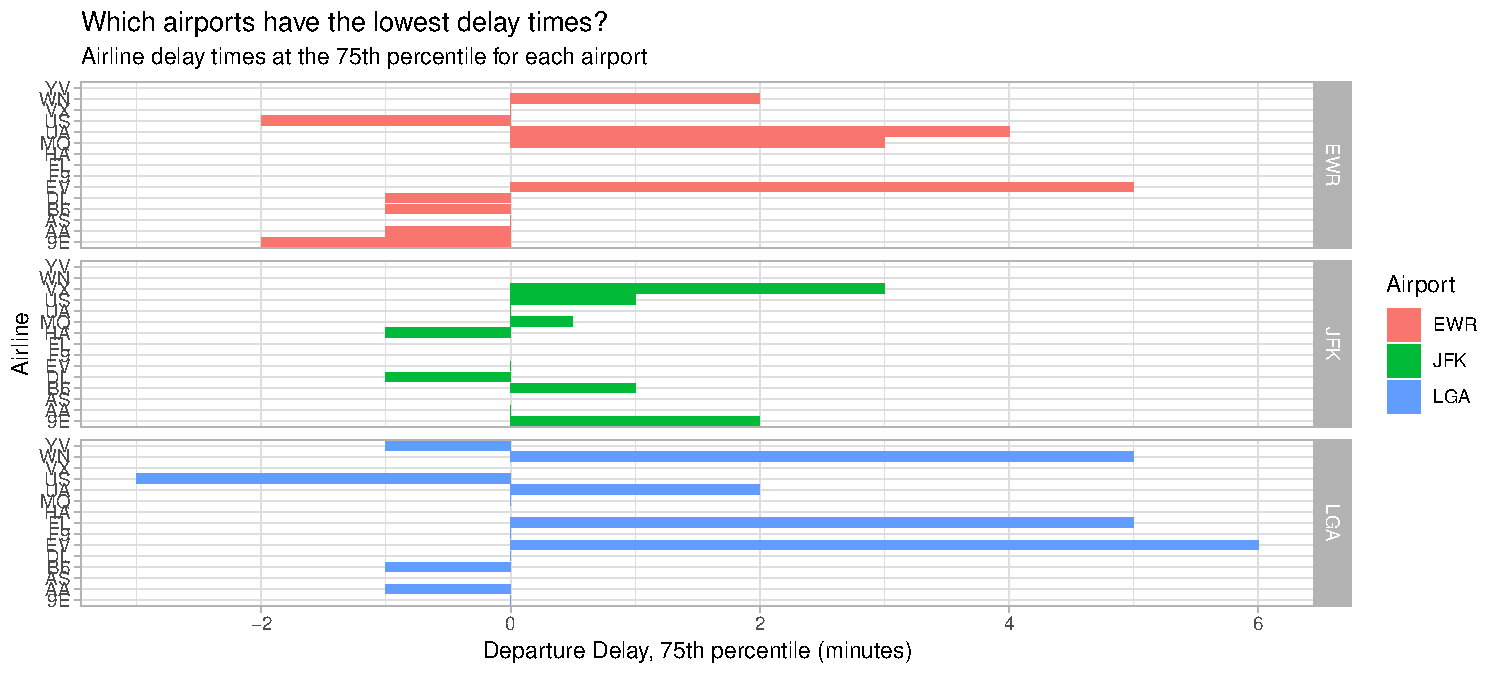
\includegraphics{case_study_03_files/figure-latex/unnamed-chunk-2-1.pdf}

\begin{Shaded}
\begin{Highlighting}[]
\CommentTok{#ggsave("plot1.png", plot = percentile_plot, width = 15, height = 5, units = "in")}
\end{Highlighting}
\end{Shaded}

Each airport has several airlines with a 75th percentile departure time
equal to zero. If by ``lowest'' delay we mean closest to zero but not
negative, then there is no exact answer to the question: just pick any
two such airline for each airport. If negative values are considered
then it makes it easier. The airlines with the lowest delay values (75th
percentile) are:

\begin{itemize}
\tightlist
\item
  EWR: US Airways and Endeavor Air
\item
  JFK: Hawaiin Airlines and Delta Air Lines
\item
  LGA: US Airways, and three tied for second place (Mesa Airlines,
  American Airlines, and JetBlue Airways)
\end{itemize}

\subsubsection{Question 2}\label{question-2}

\emph{Which origin airport is best to minimize my chances of a late
arrival when I am using Delta Airlines?}

I began by building a five-number-summary for Delta late arrivals per
airport. While the numbers here may have been sufficient enough, I also
created density plots for each airport. The densities reveal that delay
times for JFK are overall less than for the other two airports.

This is the five-number summary of the data:

\begin{Shaded}
\begin{Highlighting}[]
\CommentTok{# Use this R-Chunk to clean & wrangle your data!}
\CommentTok{# five-number summary for each airport + standard deviation}
\KeywordTok{library}\NormalTok{(pander)}
\NormalTok{flights }\OperatorTok
\StringTok{  }\KeywordTok{filter}\NormalTok{(carrier }\OperatorTok{==}\StringTok{ "DL"}\NormalTok{) }\OperatorTok
\StringTok{  }\KeywordTok{group_by}\NormalTok{(origin) }\OperatorTok
\StringTok{  }\KeywordTok{summarise}\NormalTok{(}\DataTypeTok{min =} \KeywordTok{summary}\NormalTok{(arr_delay)[}\DecValTok{1}\NormalTok{],}
            \DataTypeTok{q1 =} \KeywordTok{summary}\NormalTok{(arr_delay)[}\DecValTok{2}\NormalTok{],}
            \DataTypeTok{med =} \KeywordTok{summary}\NormalTok{(arr_delay)[}\DecValTok{3}\NormalTok{],}
            \DataTypeTok{mean =}\NormalTok{ (arr_delay)[}\DecValTok{4}\NormalTok{],}
            \DataTypeTok{q3 =} \KeywordTok{summary}\NormalTok{(arr_delay)[}\DecValTok{5}\NormalTok{],}
            \DataTypeTok{max =} \KeywordTok{summary}\NormalTok{(arr_delay)[}\DecValTok{6}\NormalTok{],}
            \DataTypeTok{sd =} \KeywordTok{sd}\NormalTok{(arr_delay, }\DataTypeTok{na.rm =} \OtherTok{TRUE}\NormalTok{)) }\OperatorTok
\StringTok{  }\KeywordTok{pander}\NormalTok{()}
\end{Highlighting}
\end{Shaded}

\begin{longtable}[]{@{}cccccccc@{}}
\toprule
\begin{minipage}[b]{0.10\columnwidth}\centering\strut
origin\strut
\end{minipage} & \begin{minipage}[b]{0.07\columnwidth}\centering\strut
min\strut
\end{minipage} & \begin{minipage}[b]{0.07\columnwidth}\centering\strut
q1\strut
\end{minipage} & \begin{minipage}[b]{0.07\columnwidth}\centering\strut
med\strut
\end{minipage} & \begin{minipage}[b]{0.08\columnwidth}\centering\strut
mean\strut
\end{minipage} & \begin{minipage}[b]{0.05\columnwidth}\centering\strut
q3\strut
\end{minipage} & \begin{minipage}[b]{0.07\columnwidth}\centering\strut
max\strut
\end{minipage} & \begin{minipage}[b]{0.08\columnwidth}\centering\strut
sd\strut
\end{minipage}\tabularnewline
\midrule
\endhead
\begin{minipage}[t]{0.10\columnwidth}\centering\strut
EWR\strut
\end{minipage} & \begin{minipage}[t]{0.07\columnwidth}\centering\strut
-54\strut
\end{minipage} & \begin{minipage}[t]{0.07\columnwidth}\centering\strut
-14\strut
\end{minipage} & \begin{minipage}[t]{0.07\columnwidth}\centering\strut
-4\strut
\end{minipage} & \begin{minipage}[t]{0.08\columnwidth}\centering\strut
43\strut
\end{minipage} & \begin{minipage}[t]{0.05\columnwidth}\centering\strut
10\strut
\end{minipage} & \begin{minipage}[t]{0.07\columnwidth}\centering\strut
847\strut
\end{minipage} & \begin{minipage}[t]{0.08\columnwidth}\centering\strut
52.19\strut
\end{minipage}\tabularnewline
\begin{minipage}[t]{0.10\columnwidth}\centering\strut
JFK\strut
\end{minipage} & \begin{minipage}[t]{0.07\columnwidth}\centering\strut
-71\strut
\end{minipage} & \begin{minipage}[t]{0.07\columnwidth}\centering\strut
-23\strut
\end{minipage} & \begin{minipage}[t]{0.07\columnwidth}\centering\strut
-11\strut
\end{minipage} & \begin{minipage}[t]{0.08\columnwidth}\centering\strut
3\strut
\end{minipage} & \begin{minipage}[t]{0.05\columnwidth}\centering\strut
5\strut
\end{minipage} & \begin{minipage}[t]{0.07\columnwidth}\centering\strut
931\strut
\end{minipage} & \begin{minipage}[t]{0.08\columnwidth}\centering\strut
41.31\strut
\end{minipage}\tabularnewline
\begin{minipage}[t]{0.10\columnwidth}\centering\strut
LGA\strut
\end{minipage} & \begin{minipage}[t]{0.07\columnwidth}\centering\strut
-58\strut
\end{minipage} & \begin{minipage}[t]{0.07\columnwidth}\centering\strut
-18\strut
\end{minipage} & \begin{minipage}[t]{0.07\columnwidth}\centering\strut
-7\strut
\end{minipage} & \begin{minipage}[t]{0.08\columnwidth}\centering\strut
-18\strut
\end{minipage} & \begin{minipage}[t]{0.05\columnwidth}\centering\strut
9\strut
\end{minipage} & \begin{minipage}[t]{0.07\columnwidth}\centering\strut
915\strut
\end{minipage} & \begin{minipage}[t]{0.08\columnwidth}\centering\strut
45.16\strut
\end{minipage}\tabularnewline
\bottomrule
\end{longtable}

\begin{Shaded}
\begin{Highlighting}[]
\NormalTok{flights }\OperatorTok
\StringTok{  }\KeywordTok{filter}\NormalTok{(carrier }\OperatorTok{==}\StringTok{ "DL"}\NormalTok{) }\OperatorTok
\StringTok{  }\KeywordTok{group_by}\NormalTok{(origin) }\OperatorTok
\StringTok{  }\KeywordTok{summarise}\NormalTok{(}\DataTypeTok{min =} \KeywordTok{summary}\NormalTok{(arr_delay)[}\DecValTok{1}\NormalTok{],}
            \DataTypeTok{q1 =} \KeywordTok{summary}\NormalTok{(arr_delay)[}\DecValTok{2}\NormalTok{],}
            \DataTypeTok{med =} \KeywordTok{summary}\NormalTok{(arr_delay)[}\DecValTok{3}\NormalTok{],}
            \DataTypeTok{mean =}\NormalTok{ (arr_delay)[}\DecValTok{4}\NormalTok{],}
            \DataTypeTok{q3 =} \KeywordTok{summary}\NormalTok{(arr_delay)[}\DecValTok{5}\NormalTok{]) }\OperatorTok
\StringTok{  }\KeywordTok{gather}\NormalTok{(}\StringTok{'min'}\NormalTok{, }\StringTok{'q1'}\NormalTok{, }\StringTok{'med'}\NormalTok{, }\StringTok{'mean'}\NormalTok{, }\StringTok{'q3'}\NormalTok{, }\DataTypeTok{key =} \StringTok{"stat"}\NormalTok{, }\DataTypeTok{value =} \StringTok{"arr_delay"}\NormalTok{, }
         \DataTypeTok{convert =} \OtherTok{TRUE}\NormalTok{) }\OperatorTok
\StringTok{  }\KeywordTok{ggplot}\NormalTok{(}\KeywordTok{aes}\NormalTok{(}\DataTypeTok{x =} \KeywordTok{factor}\NormalTok{(stat, }\DataTypeTok{levels =} \KeywordTok{c}\NormalTok{(}\StringTok{'min'}\NormalTok{, }\StringTok{'q1'}\NormalTok{, }\StringTok{'mean'}\NormalTok{, }\StringTok{'med'}\NormalTok{,}\StringTok{'q3'}\NormalTok{)),}
             \DataTypeTok{y =}\NormalTok{ arr_delay, }\DataTypeTok{group =}\NormalTok{ origin, }
             \DataTypeTok{color =}\NormalTok{ origin)) }\OperatorTok{+}
\StringTok{  }\KeywordTok{geom_point}\NormalTok{(}\DataTypeTok{size =} \DecValTok{2}\NormalTok{) }\OperatorTok{+}
\StringTok{  }\KeywordTok{geom_line}\NormalTok{(}\DataTypeTok{size =} \DecValTok{1}\NormalTok{) }\OperatorTok{+}
\StringTok{  }\KeywordTok{labs}\NormalTok{(}\DataTypeTok{title =} \StringTok{"Summary of Arrival Delay Times by Airport"}\NormalTok{, }
       \DataTypeTok{subtitle =} \StringTok{"Descriptive statistics for each airport including: }
\StringTok{       minimum, 1st quartile, median, mean, and 3rd quartile"}\NormalTok{, }
       \DataTypeTok{x =} \StringTok{"Statistic"}\NormalTok{, }
       \DataTypeTok{y =} \StringTok{"Delay of Arrival Time (minutes)"}\NormalTok{, }
       \DataTypeTok{color =} \StringTok{"Airport"}\NormalTok{)}
\end{Highlighting}
\end{Shaded}

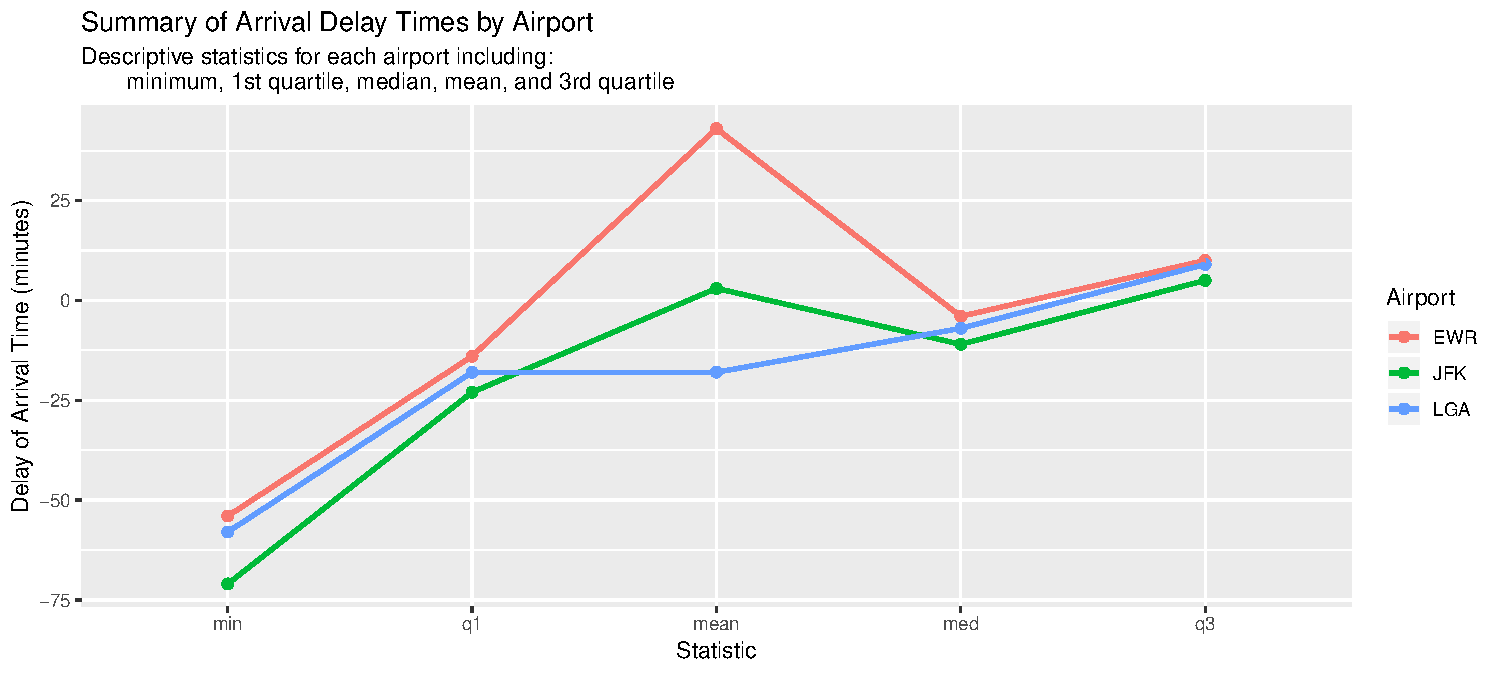
\includegraphics{case_study_03_files/figure-latex/unnamed-chunk-3-1.pdf}

\(~\)

\begin{Shaded}
\begin{Highlighting}[]
\NormalTok{flights }\OperatorTok
\StringTok{  }\KeywordTok{filter}\NormalTok{(carrier }\OperatorTok{==}\StringTok{ "DL"}\NormalTok{, }\OperatorTok{!}\KeywordTok{is.na}\NormalTok{(arr_delay)) }\OperatorTok
\StringTok{  }\KeywordTok{ggplot}\NormalTok{() }\OperatorTok{+}
\StringTok{  }\KeywordTok{geom_density}\NormalTok{(}\KeywordTok{aes}\NormalTok{(}\DataTypeTok{x =}\NormalTok{ arr_delay, }\DataTypeTok{color =}\NormalTok{ origin), }\DataTypeTok{size =} \DecValTok{1}\NormalTok{) }\OperatorTok{+}
\StringTok{  }\KeywordTok{scale_x_continuous}\NormalTok{(}\DataTypeTok{limits =} \KeywordTok{c}\NormalTok{(}\OtherTok{NA}\NormalTok{, }\DecValTok{50}\NormalTok{)) }\OperatorTok{+}
\StringTok{  }\KeywordTok{labs}\NormalTok{(}\DataTypeTok{title =} \StringTok{"Comparing airports: Delta Airlines' delayed arrivals"}\NormalTok{, }
       \DataTypeTok{x =} \StringTok{"Delay in arrival (minutes)"}\NormalTok{, }
       \DataTypeTok{y =} \StringTok{"Density"}\NormalTok{,}
       \DataTypeTok{color =} \StringTok{"Origin Airport"}\NormalTok{)}
\end{Highlighting}
\end{Shaded}

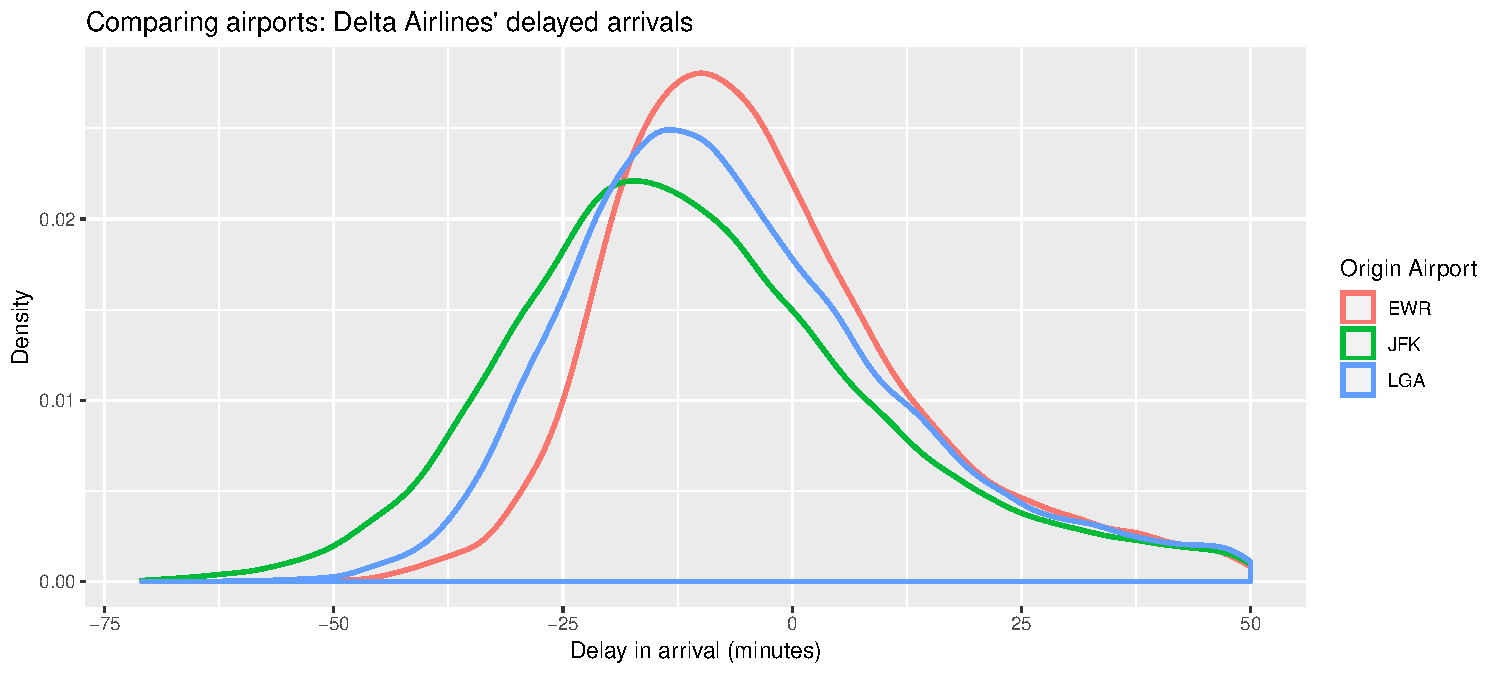
\includegraphics{case_study_03_files/figure-latex/unnamed-chunk-4-1.pdf}

The only statistic for JFK that is not smaller than the other airports
is the mean. This tells us that JFK has a more skewed distribution of
delay times than the other airports. Since JFK has the smallest values
out of the three airports for the median, 1st and 3rd quartiles, I feel
safe concluding that JFK is the best airport to choose if I want to
minimize my chances of a late arrival with Delta.

\(~\)

\subsubsection{Question 3}\label{question-3}

\emph{Which destination airport is the worst airport for arrival time?}

To answer this question I again looked at arrival delay times. The
process here was to filter the data until we got the worst of the worst
destination airports, then use those to create a graph that hopefully
displays the very worst option. Firstly, I excluded airports with less
than 50 flights since their summary statistics are probably not as
reliable, and the chances of anyone wanting to book a flight there is
small anyway. I then ran two passes to filter the data based on the
worst arrival delay times (see code for the specifics).

\begin{Shaded}
\begin{Highlighting}[]
\CommentTok{# filter airports with lesss than 50 flights}
\NormalTok{valid_dest <-}\StringTok{ }\NormalTok{flights }\OperatorTok
\StringTok{  }\KeywordTok{filter}\NormalTok{(}\OperatorTok{!}\KeywordTok{is.na}\NormalTok{(dest), }\OperatorTok{!}\KeywordTok{is.na}\NormalTok{(arr_delay)) }\OperatorTok
\StringTok{  }\KeywordTok{count}\NormalTok{(dest) }\OperatorTok
\StringTok{  }\KeywordTok{filter}\NormalTok{(n }\OperatorTok{>}\StringTok{ }\DecValTok{50}\NormalTok{) }\OperatorTok
\StringTok{  }\KeywordTok{pull}\NormalTok{(dest)}

\CommentTok{# 1st pass: exclude airports where the median, 1st and 3nd quartile are less than the mean of each of these statistics}
\NormalTok{filtered_dest <-}\StringTok{ }\NormalTok{flights }\OperatorTok
\StringTok{  }\KeywordTok{filter}\NormalTok{(}\OperatorTok{!}\KeywordTok{is.na}\NormalTok{(dest), }\OperatorTok{!}\KeywordTok{is.na}\NormalTok{(arr_delay), dest }\OperatorTok\StringTok{ }\NormalTok{valid_dest) }\OperatorTok
\StringTok{  }\KeywordTok{group_by}\NormalTok{(dest) }\OperatorTok
\StringTok{  }\KeywordTok{summarise}\NormalTok{(}\DataTypeTok{q25 =} \KeywordTok{quantile}\NormalTok{(arr_delay, .}\DecValTok{25}\NormalTok{),}
            \DataTypeTok{median =} \KeywordTok{median}\NormalTok{(arr_delay), }
            \DataTypeTok{q75 =} \KeywordTok{quantile}\NormalTok{(arr_delay, .}\DecValTok{75}\NormalTok{)) }\OperatorTok
\StringTok{  }\KeywordTok{filter}\NormalTok{(q25 }\OperatorTok{>}\StringTok{ }\KeywordTok{mean}\NormalTok{(q25), }
\NormalTok{         median }\OperatorTok{>}\StringTok{ }\KeywordTok{mean}\NormalTok{(median),}
\NormalTok{         q75 }\OperatorTok{>}\StringTok{ }\KeywordTok{mean}\NormalTok{(q75)) }\OperatorTok
\StringTok{  }\KeywordTok{pull}\NormalTok{(dest)}

\CommentTok{# 2nd pass: of the remaining airports, exclude those whose median delay time is less than the median of the remaining airports' median delay time}
\NormalTok{filtered_dest2 <-}\StringTok{ }\NormalTok{flights }\OperatorTok
\StringTok{  }\KeywordTok{filter}\NormalTok{(}\OperatorTok{!}\KeywordTok{is.na}\NormalTok{(dest), }\OperatorTok{!}\KeywordTok{is.na}\NormalTok{(arr_delay), dest }\OperatorTok\StringTok{ }\NormalTok{filtered_dest) }\OperatorTok
\StringTok{  }\KeywordTok{group_by}\NormalTok{(dest) }\OperatorTok
\StringTok{  }\KeywordTok{summarise}\NormalTok{(}\DataTypeTok{median =} \KeywordTok{median}\NormalTok{(arr_delay)) }\OperatorTok
\StringTok{  }\KeywordTok{filter}\NormalTok{(median }\OperatorTok{>}\StringTok{ }\KeywordTok{median}\NormalTok{(median)) }\OperatorTok
\StringTok{  }\KeywordTok{pull}\NormalTok{(dest)}
\end{Highlighting}
\end{Shaded}

The very worst airports in regard to arrival delays are in the boxplot
below:

\begin{Shaded}
\begin{Highlighting}[]
\NormalTok{cae <-}\StringTok{ }\NormalTok{flights }\OperatorTok
\StringTok{  }\KeywordTok{filter}\NormalTok{(}\OperatorTok{!}\KeywordTok{is.na}\NormalTok{(dest), }\OperatorTok{!}\KeywordTok{is.na}\NormalTok{(arr_delay), dest }\OperatorTok\StringTok{ "CAE"}\NormalTok{) }\OperatorTok
\StringTok{  }\KeywordTok{select}\NormalTok{(dest, arr_delay)}

\NormalTok{flights }\OperatorTok
\StringTok{  }\KeywordTok{filter}\NormalTok{(}\OperatorTok{!}\KeywordTok{is.na}\NormalTok{(dest), }\OperatorTok{!}\KeywordTok{is.na}\NormalTok{(arr_delay), dest }\OperatorTok\StringTok{ }\NormalTok{filtered_dest2) }\OperatorTok
\StringTok{  }\KeywordTok{select}\NormalTok{(dest, arr_delay) }\OperatorTok
\StringTok{  }\KeywordTok{ggplot}\NormalTok{() }\OperatorTok{+}
\StringTok{  }\KeywordTok{geom_boxplot}\NormalTok{(}\KeywordTok{aes}\NormalTok{(}\DataTypeTok{x =}\NormalTok{ dest, }\DataTypeTok{y =}\NormalTok{ arr_delay)) }\OperatorTok{+}
\StringTok{  }\KeywordTok{geom_boxplot}\NormalTok{(}\DataTypeTok{data =}\NormalTok{ cae, }\KeywordTok{aes}\NormalTok{(}\DataTypeTok{x =}\NormalTok{ dest, }\DataTypeTok{y =}\NormalTok{ arr_delay), }\DataTypeTok{fill =} \StringTok{"tomato1"}\NormalTok{) }\OperatorTok{+}
\StringTok{  }\KeywordTok{scale_y_continuous}\NormalTok{(}\DataTypeTok{limits =} \KeywordTok{c}\NormalTok{(}\OperatorTok{-}\DecValTok{20}\NormalTok{, }\DecValTok{35}\NormalTok{)) }\OperatorTok{+}
\StringTok{  }\KeywordTok{coord_flip}\NormalTok{() }\OperatorTok{+}
\StringTok{  }\KeywordTok{theme_dark}\NormalTok{() }\OperatorTok{+}
\StringTok{  }\KeywordTok{labs}\NormalTok{(}\DataTypeTok{title =} \StringTok{"Airports with the longest delays for arriving flights"}\NormalTok{,}
       \DataTypeTok{subtitle =} \StringTok{"The worst offender is highlighted in red: Columbia Metropolitan"}\NormalTok{,}
       \DataTypeTok{y =} \StringTok{"Arrival delays (minutes)"}\NormalTok{,}
       \DataTypeTok{x =} \StringTok{"Airport"}\NormalTok{)}
\end{Highlighting}
\end{Shaded}

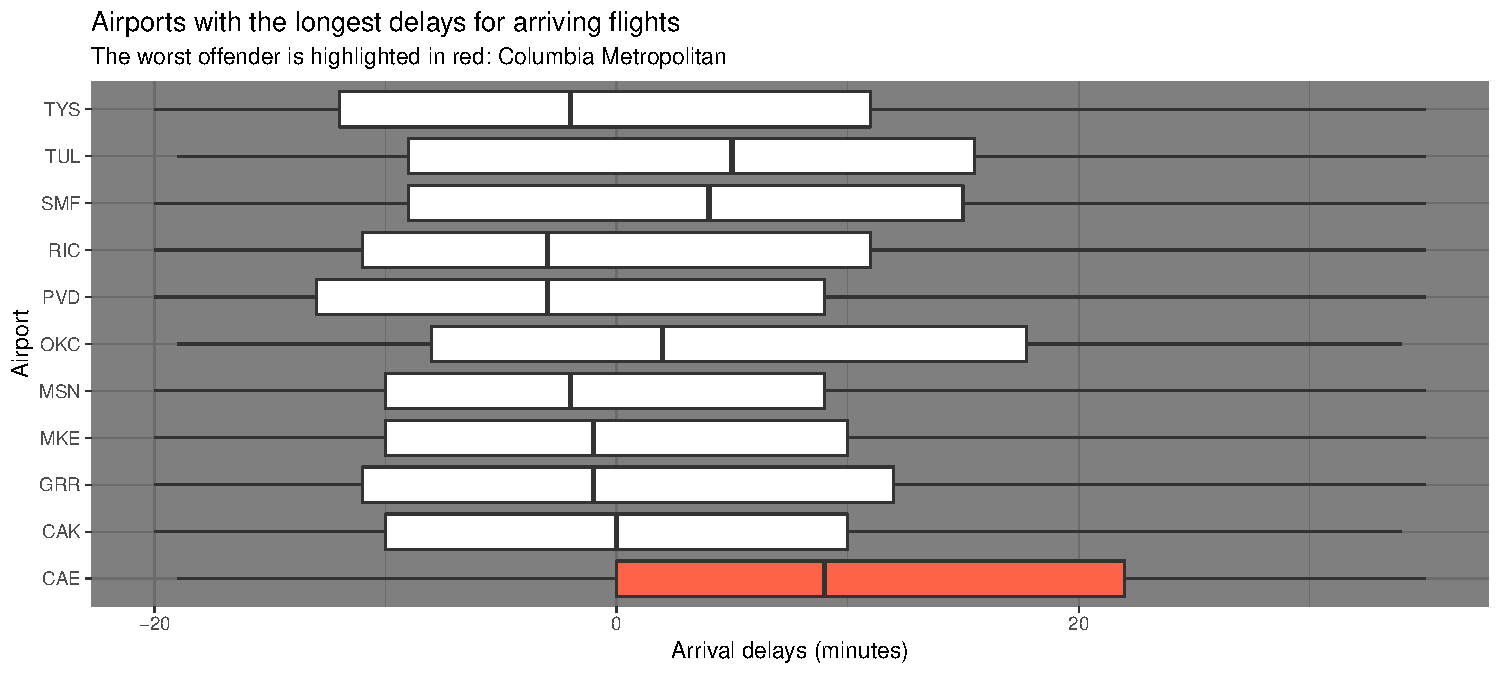
\includegraphics{case_study_03_files/figure-latex/unnamed-chunk-6-1.pdf}

Conveniently, one airport stands out among the others as having the
highest of all delay times: \textbf{Columbia Metropolitan (CAE)}. Not
only does it have the highest median delay time, but surpringly the
highest delay time at the 1st and 3rd quantiles too. It has a
\textbf{median delay time of 28 minutes}, and an even worse mean at 41.8
minutes.

\(~\)


\end{document}
